% Content for Chapter 5, Section 5.8 — pulled in by chapters/05-system-design.tex
\subsection{دور الخدمة ونطاقها}

% CH2-REF: originally ended "الموصوفة نظريًّا في القسم~\ref{sec:knowledge-pipeline}." — restore with chapter 2.
تحوّل خدمة المعرفة المواد المرجعية التي يرفعها المعلّم، من ملفّات \en{PDF} ومستندات \en{Word} وعروض \en{PowerPoint}، إلى قاعدة معرفية قابلة للبحث الدلالي تغذّي قدرات التوليد المعزّز بالاسترجاع (\en{RAG}). وتنفّذ الخدمة مرحلتين: الفهرسة (\en{Indexing}) والاسترجاع (\en{Retrieval})، فيُبنى فهرس دلالي لكل فصل دراسي تُؤصَّل به إجابات النظام في مادة ذلك الفصل.

\subsection{مكوّنات الخدمة}

يعرض الشكل~\ref{fig:comp-05} مكوّنات الخدمة وروابطها الخارجية، وهي مجمّعة بحسب المهامّ الأربع التي تؤدّيها: الاستيعاب والاسترجاع والتلخيص وإعادة التضمين.

\begin{figure}[htbp]
  \centering
  % Width to be re-checked when the draw.io export replaces this PNG.
  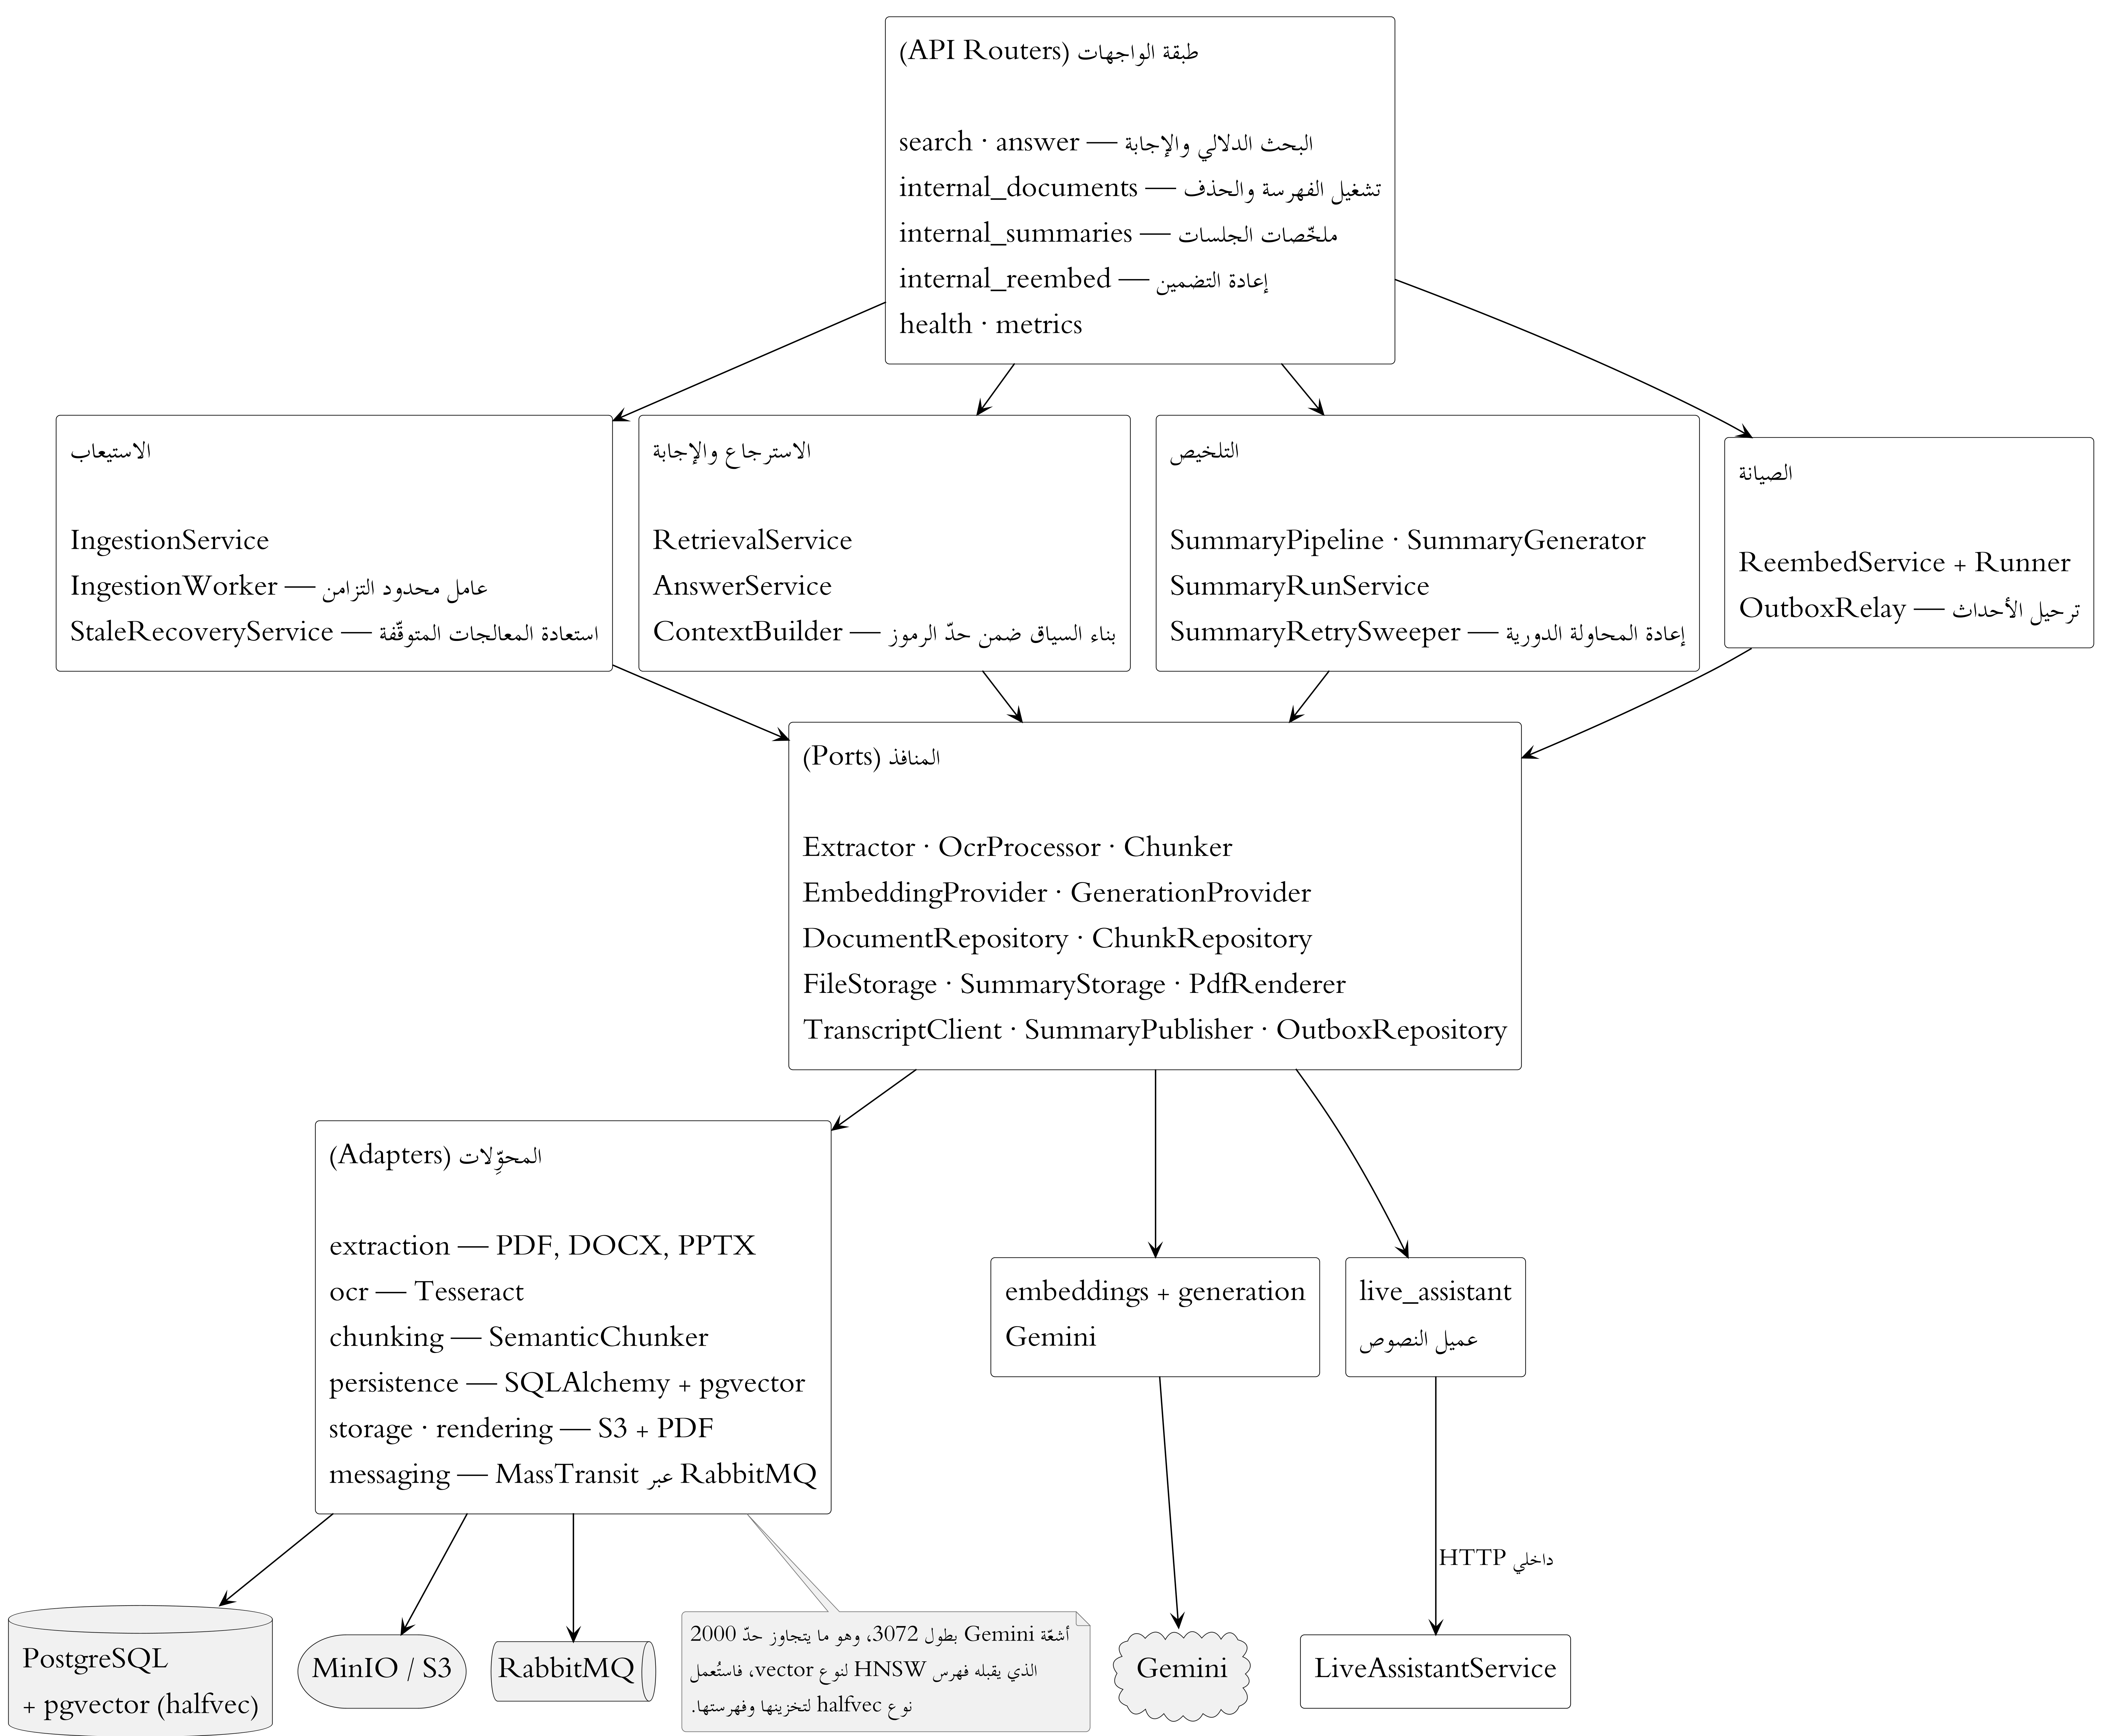
\includegraphics[width=\textwidth,height=0.8\textheight,keepaspectratio]{figures/comp-05-rag.png}
  \caption{مخطط مكوّنات خدمة المعرفة.}
  \label{fig:comp-05}
\end{figure}

وطُبّق في هذه الخدمة نمط المنافذ والمحوِّلات: تُعرّف طبقة التطبيق منافذ مجرّدة تصف ما تحتاجه الخدمة من استخراج وتضمين وتخزين، ويقع كل اختيار تقني خلف أحدها في طبقة البنية التحتية. ويحصر ذلك استبدال مزوّد التضمين أو محرّك التعرّف الضوئي في محوِّل واحد، دون تعديل منطق خط الأنابيب. ويعرض الشكل~\ref{fig:class-01} هذا التصميم مطبَّقاً على خط أنابيب الاستيعاب.

\begin{figure}[htbp]
  \centering
  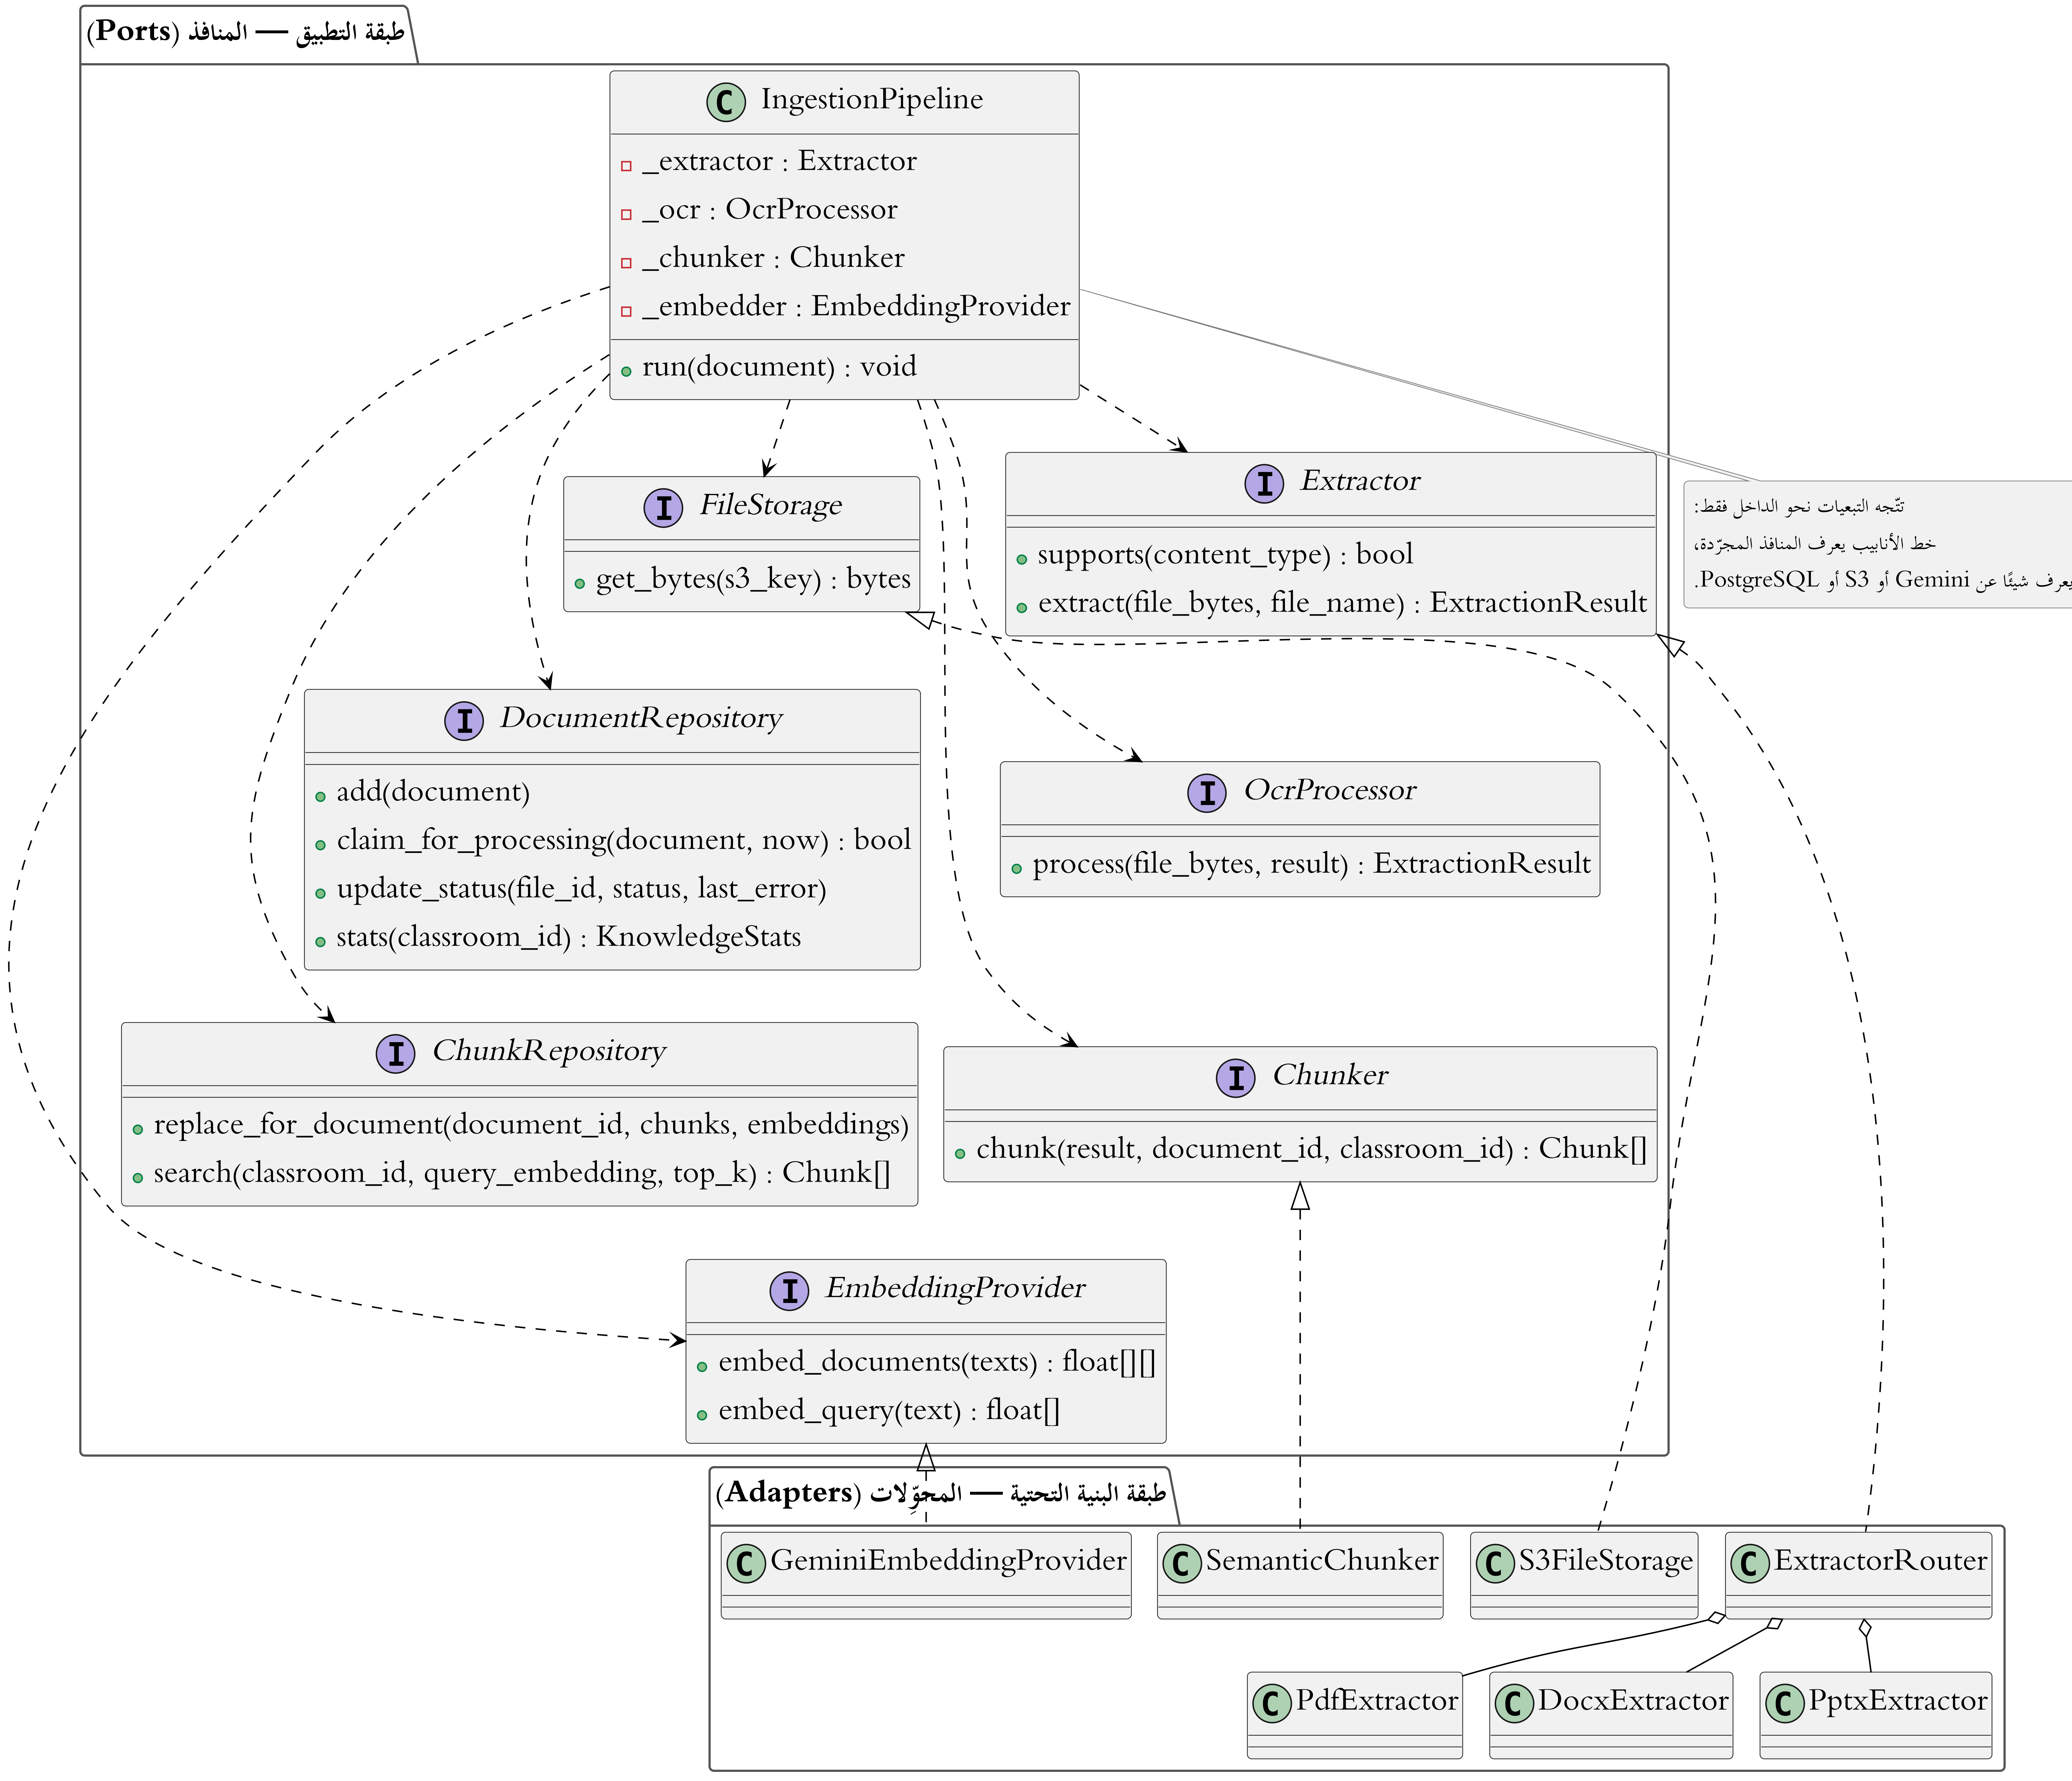
\includegraphics[width=\textwidth,height=0.8\textheight,keepaspectratio]{figures/class-01-ports-adapters.png}
  \caption{مخطط الصفوف لنمط المنافذ والمحوِّلات في خط أنابيب الاستيعاب.}
  \label{fig:class-01}
\end{figure}

\subsection{نموذج البيانات}
\label{subsec:rag-data-model}

يقوم نموذج البيانات على أربعة كيانات يعرضها الشكل~\ref{fig:erd-04}: المستند والمقطع، وسجلّات محاولات التلخيص، وجدول صندوق الصادر.

\begin{figure}[htbp]
  \centering
  % Width to be re-checked when the draw.io export replaces this PNG.
  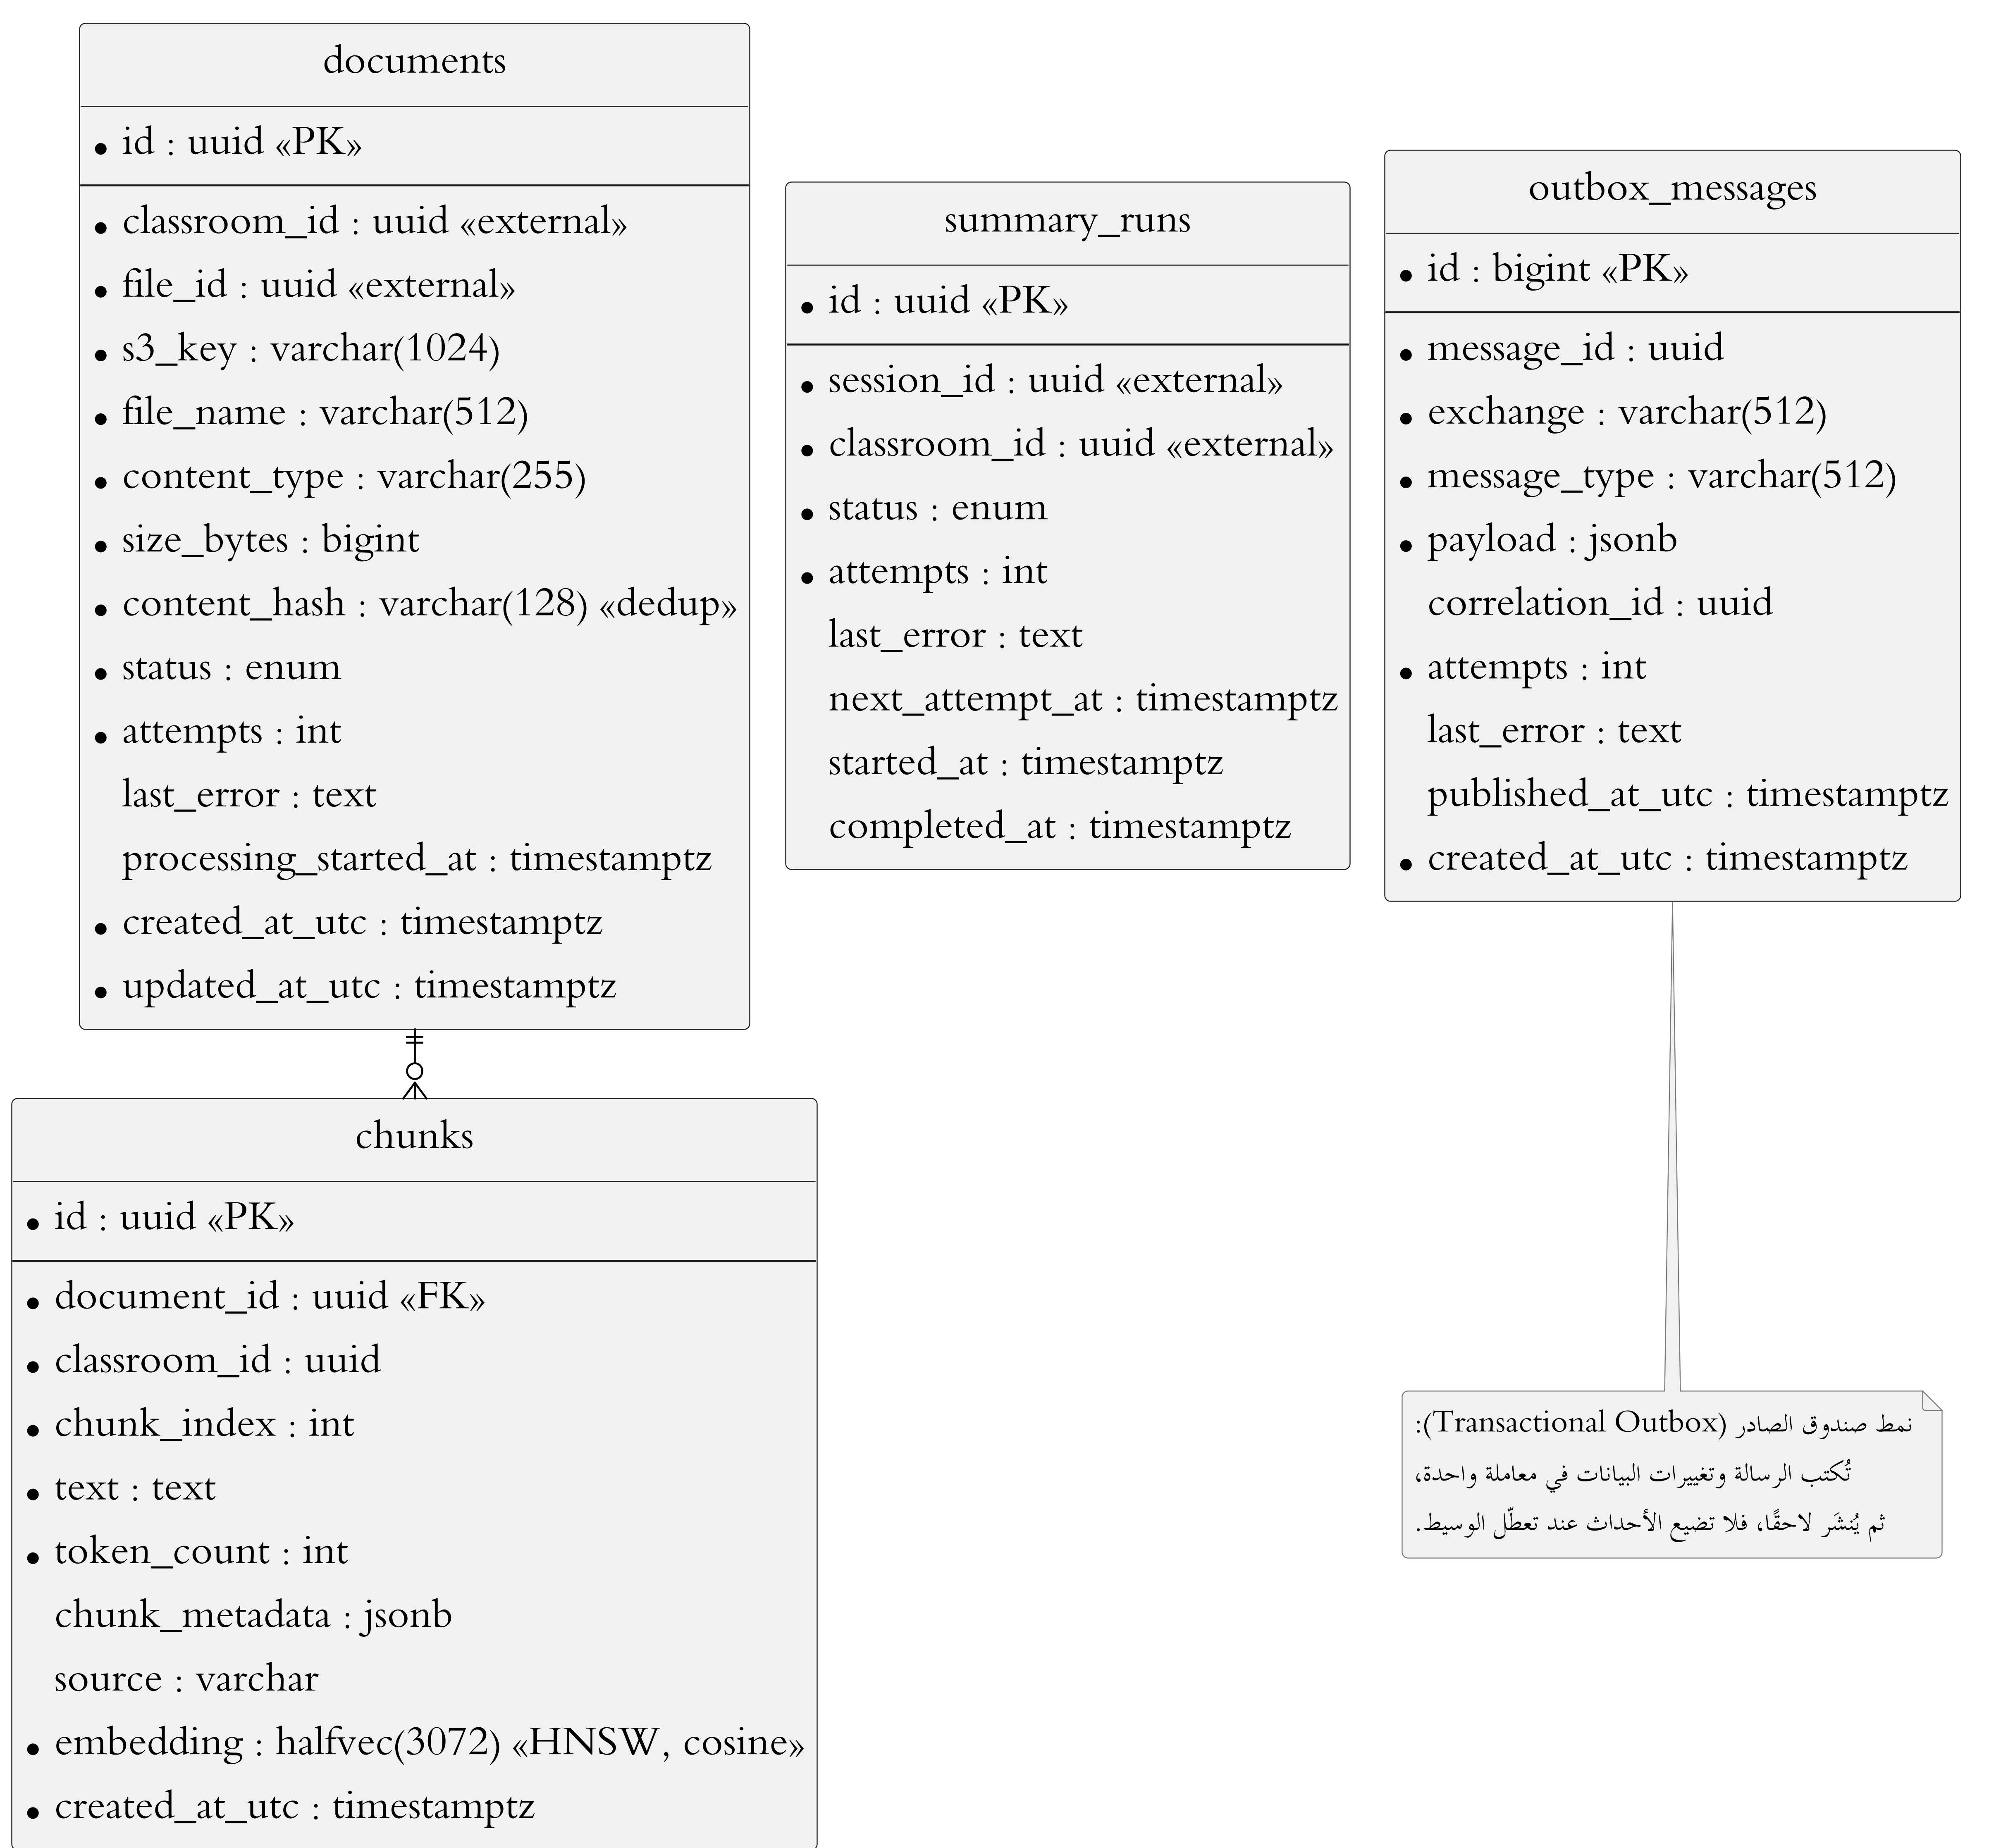
\includegraphics[width=\textwidth,height=0.8\textheight,keepaspectratio]{figures/erd-04-rag.png}
  \caption{مخطط الكيانات والعلاقات لخدمة المعرفة.}
  \label{fig:erd-04}
\end{figure}

ويتضمّن هذا النموذج قرارين تصميميين:

\begin{enumerate}
  \item \textbf{تضمين معرّف الفصل في كيان المقطع}: يتيح قصر البحث الدلالي على فصل بعينه، فيُعزَل محتوى كل فصل ولا يتسرّب إلى نتائج فصل آخر.
  \item \textbf{استعمال النوع \en{halfvec} لتخزين الأشعّة}: يبلغ طول شعاع التضمين 3072، وهو يتجاوز الحدّ الأقصى البالغ 2000 الذي يقبله فهرس \en{HNSW} للنوع \en{vector}. ويقبل النوع \en{halfvec} هذا الطول ويسمح بفهرسته.
\end{enumerate}
